\chapter{Affichage digital 7 segments}
\vspace{2cm}
\section{Énoncé}
Le but de ce challenge est de développer la fonction \texttt{digital\_time()->str} qui retourne l'heure actuelle au format d'affichage digital à sept segments\footnote{\url{https://fr.wikipedia.org/wiki/Affichage_\%C3\%A0_sept_segments}}.
\medskip

\subsection*{Étapes}
\begin{enumerate}
	\item Transcrire les chiffres de 0 à 9 en sept segments digitaux.
	\item Transcrire plusieurs chiffres à la suite sur une seule ligne.
	\item Afficher l'heure en la retranscrivant.
\end{enumerate}
\medskip

\subsection*{Conditions}
\begin{itemize}
	\item[-] L'affichage se fait via la console
	\item[-] L'heure doit être affichée au format 24h.
	\item[-] L'heure et les minutes sont séparées par deux points, le tout sur une même ligne d'affichage avec deux espaces de séparation.
	\item[-] Le résultat de l'affichage de l'heure actuelle doit correspondre aux exemples ci-dessous à l'aide du caractère \og \texttt{\#}\fg{}.
	\item[-] Les sept segments \texttt{a}, \texttt{b}, \texttt{c}, \texttt{d}, \texttt{e}, \texttt{f}, \texttt{g} sont les suivants :
	\newpage
	
	\begin{verbatim}
     a
     v 
    ####   
f-> #  # <- b
    #### <- g
e-> #  # <- c
    ####
     ^
     d
	\end{verbatim}
	\item[-] Pour des raisons d'ergonomie et d'esthétisme, les segments se superposent et s'affichent de manière plus allongée, ainsi le chiffre \texttt{2} s'affichera de la façon suivante:
	\begin{verbatim}
	
             ####                        ##
                #                          #
comme ceci : ####   et pas comme cela :  ## 
             #                          #
             ####                        ##	
	\end{verbatim}
\end{itemize}
\medskip

\subsection*{Exemples}
\begin{itemize}
	\item[-] À \texttt{17h26}, le résultat de \texttt{digital\_time()} donne :
	\begin{verbatim}
	#  ####     ####  ####
	#     #  #     #  #  
	#     #     ####  ####
	#     #  #  #     #  #
	#     #     ####  ####
	\end{verbatim}
	\medskip
	
	\item[-] À \texttt{23h59}, le résultat de \texttt{digital\_time()} donne :
	\begin{verbatim}
	####  ####     ####  ####
	   #     #  #  #     #  #
	####  ####     ####  ####
	#        #  #     #     #
	####  ####     ####  ####
	\end{verbatim}
	\medskip
	
	\item[-] À \texttt{4h08}, le résultat de \texttt{digital\_time()} donne :
-	\begin{verbatim}
	#  #     ####  ####
	#  #  #  #  #  #  #
	####     #  #  ####
	   #  #  #  #  #  #
	   #     ####  ####
	\end{verbatim}
\end{itemize}
\medskip

\section{Ma proposition avec l'utilisation de \texttt{Numpy}}
\begin{lstlisting}
from numpy import hstack, delete, full, ndarray
from datetime import datetime

SEG_MAP = (((0, 0), (0, 1), (0, 2), (0, 3)),  # a
           ((0, 3), (1, 3), (2, 3)),  # b
           ((2, 3), (3, 3), (4, 3)),  # c
           ((4, 0), (4, 1), (4, 2), (4, 3)),  # d
           ((4, 0), (3, 0), (2, 0)),  # e
           ((2, 0), (1, 0), (0, 0)),  # f
           ((2, 0), (2, 1), (2, 2), (2, 3)),  # g
           ((1, 0), (3, 0)))


def display(el: str) -> ndarray:
    digit = full((5, 6), [" "], dtype=str)
    match el:
        case " ": return digit
        case ":":
            s = [*[0]*7, 1]
            digit = delete(digit, slice(3), 1)
        case _:
            b = [int(b) for b in f"{int(el):04b}"][::-1]
            s = (b[3] or b[1] or b[0] and b[2] or not b[0]
                 and not b[2],
                 b[0] and b[1] or not b[1] and not b[0]
                 or not b[2],
                 b[2] or b[3] or not b[1] or b[0],
                 b[3] or b[1] and not b[0] or not b[2]
                 and not b[0] or not b[1] and b[0] and b[2]
                 or b[1] and not b[2],
                 b[1] and not b[0] or not b[0]
                 and not b[2],
                 b[3] or not b[0] and b[2] or not b[1]
                 and b[2] or not b[1] and not b[0],
                 b[3] or b[1] and not b[0] or not b[1]
                 and b[2] or not b[2] and b[1])
    digit[*zip(*[(r, c) for i, el in enumerate(s) if el
                 for r, c in SEG_MAP[i]])] = "#"
    return digit


def digital_time():
    time = datetime.now().strftime("%H:%M").lstrip("0")
    return "\n".join("".join(r) for r in
                     hstack([display(el) for el in
                             (time if len(time) == 5 else 
                              " " + time)]))


if __name__ == "__main__":
    print(digital_time())
\end{lstlisting}
\medskip

\section{Explications}
\subsection*{Contexte}
Il s'agit de trouver le moyen d'afficher un nombre sous forme digitale en sept segments comme on peut le voir sur certaines horloges numériques, puis d'afficher l'heure actuelle.
\medskip

\subsection*{Différentes problématiques}
\begin{itemize}
	\item[\textbullet] \textbf{Conversion d'un chiffre en sept segments pour simuler un affichage digital}: Il s'agit de repérer la position de chacun des segments puis \og d'allumer\fg{} les segments spécifiques au chiffre à afficher.
	\medskip
	
	\item[\textbullet] \textbf{Afficher plusieurs chiffres sur une ligne}: L'étape suivante est d'afficher plusieurs chiffres sur une même ligne en transposant les \og matrices\fg{} des chiffres à afficher.
	\medskip
	
	\item[\textbullet] \textbf{Ajouter le séparateur heure/minute}: Il nous faut donc ajouter le caractère \og \texttt{:}\fg{} entre les heures et les minutes.
	\medskip
	
	\item[\textbullet] \textbf{Formatage particulier}: Les heures de 0 à 9 ne doivent pas afficher un zéro mais laisser l'espace d'un \textit{digit} à gauche.
\end{itemize}
\medskip

\subsection*{Explication du code}
Le code se divise en trois, voire quatre parties :
\medskip

\subsubsection*{\textbullet{} Définir les segments à allumer en fonction du chiffre à afficher}
Ma méthode ici consiste à chercher des solutions combinatoires pour chaque segment en fonction du chiffre à afficher. Les chiffres sont au nombre de 10 et peuvent varier de 0 à 9. Ce qui nécessite quatre \textit{bits} pour les coder en binaire :
\begin{verbatim}
0000 -> 0
0001 -> 1
0010 -> 2
...
1000 -> 8
1001 -> 9
\end{verbatim}
\medskip

Il y a ensuite sept solutions combinatoires à rechercher pour chacun des segments de \og \texttt{a}\fg{} à \og \texttt{g}\fg{}.
\begin{figure}[h]
    \centering
    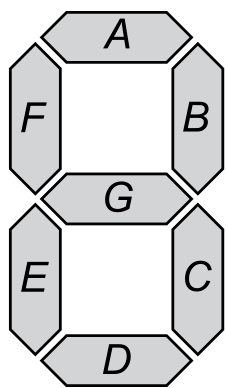
\includegraphics[width=0.2\textwidth]{IMG/sept_segments.png}
    \caption{Représentation visuelle des sept solutions combinatoires}
    \label{fig:colorpicker}
\end{figure}
\medskip

Ainsi il faut allumer les segments \texttt{B} et \texttt{C} pour coder le chiffre \texttt{1}, \texttt{BCFG} pour le chiffre \texttt{4}, \texttt{ABCDEF} pour le chiffre \texttt{0}, etc. On peut donc poser tous ces résultat dans une \textit{table de vérité} :
\begin{figure}[h]
    \centering
    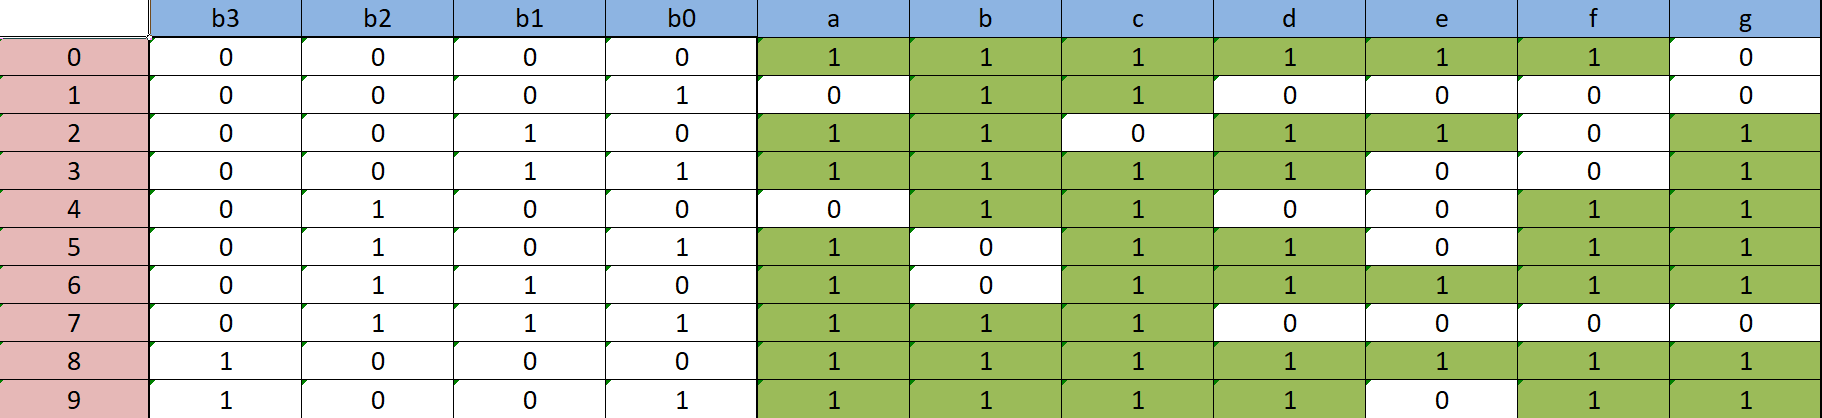
\includegraphics[width=0.9\textwidth]{IMG/table_de_verite.png}
    \caption{\textit{Table de vérité}}
    \label{fig:colorpicker}
\end{figure}
\medskip

A gauche les chiffres transcrits en quatre \textit{bits} de \texttt{b0} à \texttt{b3} et à droite les segments à allumer.
\medskip

La table de vérité est incomplète dans le sens où on n'utilise pas la totalité des possibilités en quatre \textit{bits}. Ainsi, on pourra être libre de choisir n'importe quels états durant la simplification de nos équations à l'aide des \textit{tableaux de Karnaugh} (ces combinaisons seront notées en rouge dans les tableaux).
\medskip

Le chiffre est d'abord converti en binaire sur quatre \textit{bits} pour procéder au calcul avec l'\textit{algèbre de Boole }:
\begin{verbatim}
b = [int(b) for b in f"{int(el):04b}"][::-1]
\end{verbatim}
\medskip

Pour faire bien correspondre à mes tableaux je suis obliger de faire une inversion via \texttt{[::-1]}.
\newpage

Pour simplifier chacune des sept solutions on posera nos \textit{tableaux de Karnaugh}\footnote{\textit{Tableaux de Karnaugh} - simplification d'expression en \textit{algèbre de Boole}: \url{https://www.youtube.com/watch?v=2tULBk6V9ZE}} de cette manière :
\begin{figure}[h!]
    \centering
    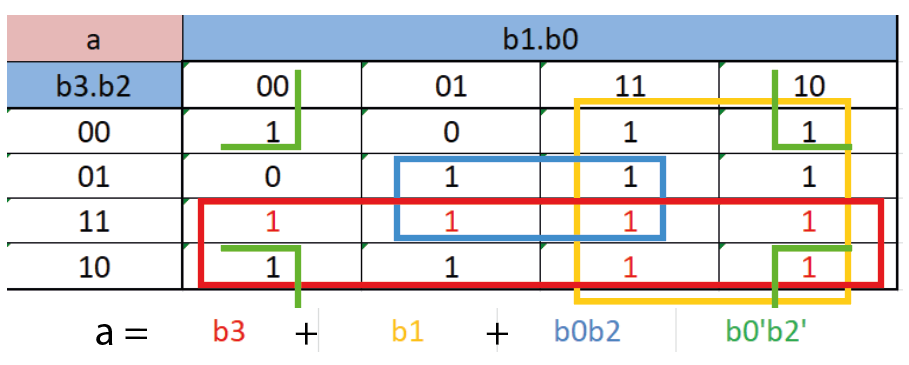
\includegraphics[width=0.9\textwidth]{IMG/tab_de_K_1.png}
    \caption{\textit{Tableau de Karnaugh} - 1}
    \label{fig:colorpicker}
\end{figure}
\medskip

\begin{figure}[h!]
    \centering
    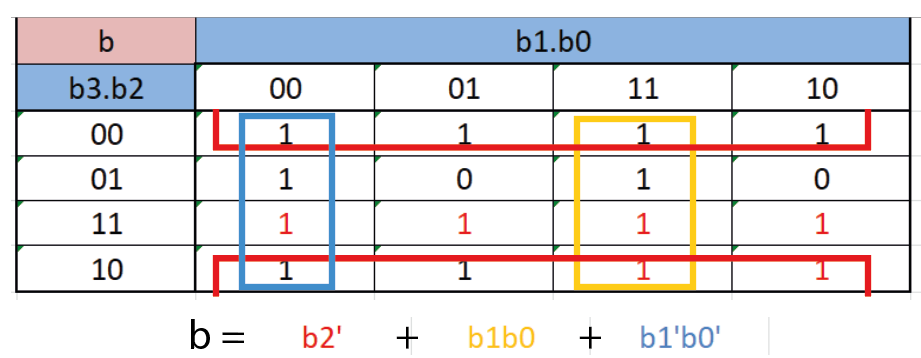
\includegraphics[width=0.9\textwidth]{IMG/tab_de_K_2.png}
    \caption{\textit{Tableau de Karnaugh} - 2}
    \label{fig:colorpicker}
\end{figure}
\medskip

\begin{figure}[h!]
    \centering
    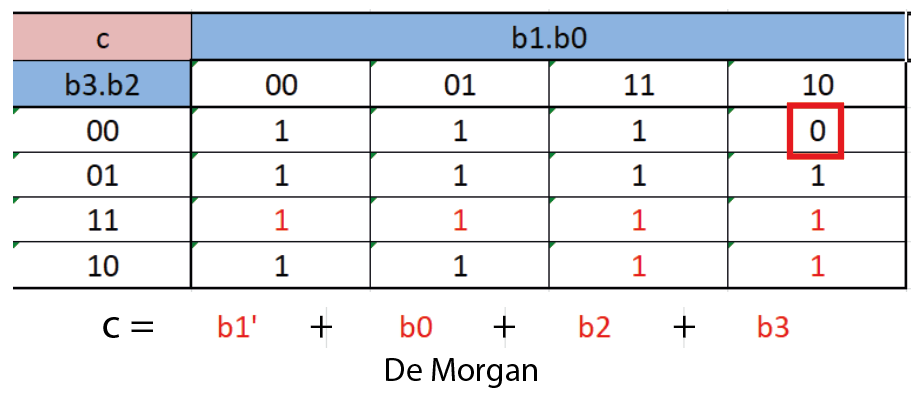
\includegraphics[width=0.9\textwidth]{IMG/tab_de_K_3.png}
    \caption{\textit{Tableau de Karnaugh} - 3}
    \label{fig:colorpicker}
\end{figure}
\newpage

\begin{figure}[h!]
    \centering
    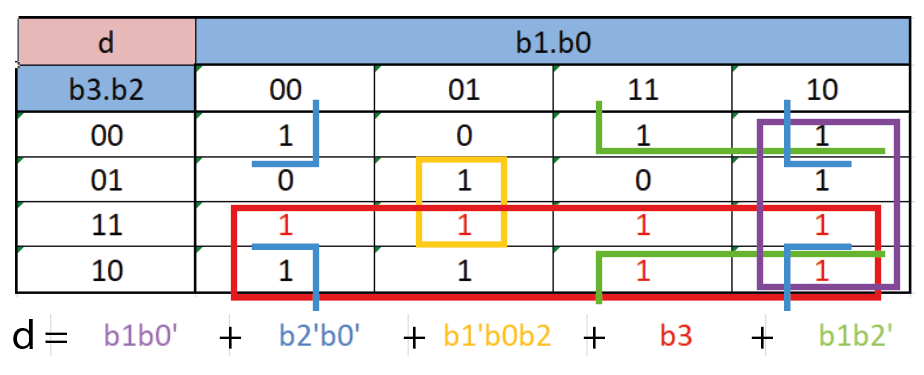
\includegraphics[width=0.9\textwidth]{IMG/tab_de_K_4.png}
    \caption{\textit{Tableau de Karnaugh} - 4}
    \label{fig:colorpicker}
\end{figure}
\medskip

\begin{figure}[h!]
    \centering
    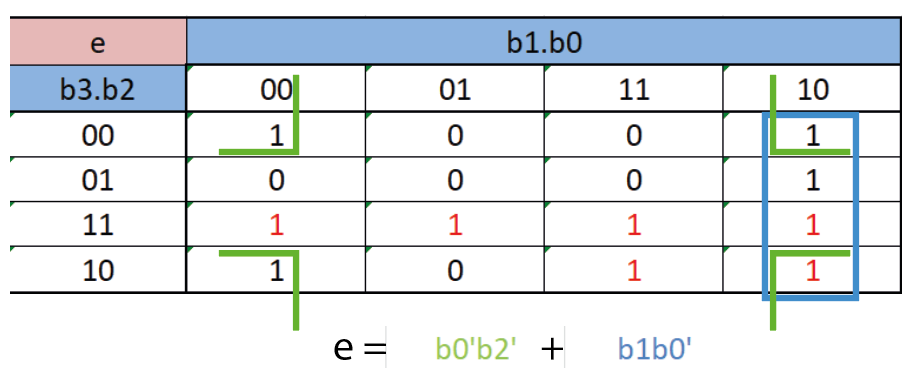
\includegraphics[width=0.9\textwidth]{IMG/tab_de_K_5.png}
    \caption{\textit{Tableau de Karnaugh} - 5}
    \label{fig:colorpicker}
\end{figure}
\medskip

\begin{figure}[h!]
    \centering
    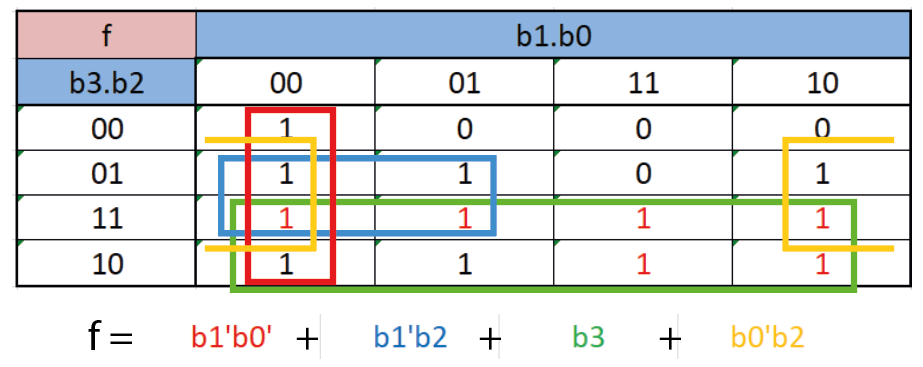
\includegraphics[width=0.9\textwidth]{IMG/tab_de_K_6.png}
    \caption{\textit{Tableau de Karnaugh} - 6}
    \label{fig:colorpicker}
\end{figure}
\newpage

\begin{figure}[h!]
    \centering
    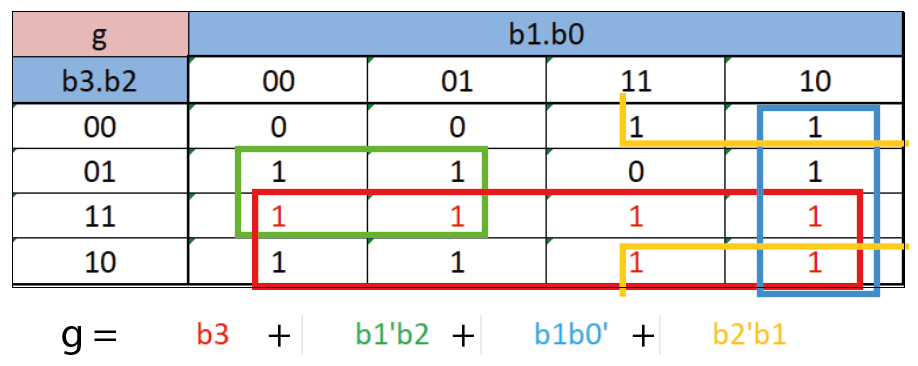
\includegraphics[width=0.9\textwidth]{IMG/tab_de_K_7.png}
    \caption{\textit{Tableau de Karnaugh} - 7}
    \label{fig:colorpicker}
\end{figure}
\medskip

On peut donc poser les solutions sous forme de listes qu'on pourra interpréter respectivement via les index de \texttt{0} à \texttt{6} pour les segments de \texttt{a} à \texttt{g}.
\begin{lstlisting}
s = (b[3] or b[1] or b[0] and b[2] or not b[0] and not 
     b[2],
     b[0] and b[1] or not b[1] and not b[0] or not b[2],
     b[2] or b[3] or not b[1] or b[0],
     b[3] or b[1] and not b[0] or not b[2] and not b[0] 
     or not b[1] and b[0] and b[2] or b[1] and not b[2],
     b[1] and not b[0] or not b[0] and not b[2],
     b[3] or not b[0] and b[2] or not b[1] and b[2] 
     or not b[1] and not b[0],
     b[3] or b[1] and not b[0] or not b[1] and b[2] 
     or not b[2] and b[1])
\end{lstlisting}
\medskip

Puis la liste \texttt{SEG\_MAP} me permet de fixer la position des segments en posant leur coordonnées dans la matrice d'un chiffre digital :
\begin{lstlisting}
SEG_MAP = (((0, 0), (0, 1), (0, 2), (0, 3)), # a
           ((0, 3), (1, 3), (2, 3)), # b
           ((2, 3), (3, 3), (4, 3)), # c
           ((4, 0), (4, 1), (4, 2), (4, 3)), # d
           ((4, 0), (3, 0), (2, 0)), # e
           ((2, 0), (1, 0), (0, 0)), # f
           ((2, 0), (2, 1), (2, 2), (2, 3)), # g
           ((1, 0), (3, 0))) # :
\end{lstlisting}
\medskip

Notez que la dernière ligne correspond au caractère de séparation \og \texttt{:}\fg{} entre l'heure et les minutes.
\medskip

\subsubsection*{\textbullet{} Affichage d'un \textit{digit}}
La variable \texttt{digit} est un tableau \textit{Numpy} initialisé avec des espaces :
\begin{verbatim}
digit = full((5, 6), [" "],dtype=str)
\end{verbatim}
\medskip

Je teste ici avec \texttt{match case} les caractères à afficher, soit \texttt{" "} pour un \textit{digit} \og éteint\fg{}, puis les deux points (\og \texttt{:}\fg{}) pour le séparateur et le reste pour les chiffres de 0 à 9.
\begin{verbatim}
match el:
        case " ": ...
        case ":":
            ...
        case _:
            ...
\end{verbatim}
\medskip

Une fois les solutions de ma table de vérité trouvées, alors on récupère les coordonnées pour afficher un \og \texttt{\#}\fg{} à chaque fois pour former les segments à allumer :
\begin{lstlisting}
digit[*zip(*[(r, c) for i, el in enumerate(s) if el
                 for r, c in SEG_MAP[i]])] = "#"
    return digit
\end{lstlisting}
\medskip

Cette fonction peut être éclatée de cette manière pour plus de lisibilité :
\begin{lstlisting}
pos = [(r, c) for i, el in enumerate(s) if el 
           for r, c in SEG_MAP[i]]
r, c = zip(*pos)
digit[r, c] = "#"
\end{lstlisting}
\medskip

Ce n'est qu'une simple transposition afin de réunir les coordonnées \texttt{x} et \texttt{y} et les appliquer d'un coup et ainsi remplir le tableau \textit{Numpy} \texttt{digit}.
\medskip

\subsubsection*{\textbullet{} Afficher sur une ligne}
Pour ce faire on doit procéder à une lecture ligne par ligne de chaque \texttt{digit}. On utilise pour cela la fonction \texttt{hstack()}\footnote{\url{https://numpy.org/doc/stable/reference/generated/numpy.hstack.html}} qui permet de concaténer ligne par ligne mes tableaux \textit{Numpy}.
\medskip

Tout se fait à cette ligne :
\begin{verbatim}
hstack([display(el) for el in time])
\end{verbatim}
\medskip

\subsubsection*{\textbullet{} Afficher l'heure en suivant l'énoncé}
L'affichage de l'heure n'est pas bien complexe: heure sur un chiffre et les minutes avec deux chiffres. Il faut penser à effacer le premier zéro de l'heure si l'heure est entre 0 et 9 puis d'ajouter un \textit{digit} blanc pour l'affichage.
\begin{lstlisting}
time = datetime.now().strftime("%H:%M").lstrip("0")
...
...time if len(time) == 5 else " "+time...
\end{lstlisting}
\medskip

Pour cela je cherche la taille de l'heure et si l'on a que cinq caractères alors on se trouve dans le cas d'un affichage avec deux \textit{digits} pour l'heure sinon ce sera une longueur de quatre :
\begin{itemize}
	\item[-] 3:24 <- une longueur de quatre
	\item[-] 15h58 <- une longueur de cinq
\end{itemize}
\medskip

Le caractère spécial \og \texttt{:}\fg{} est calculé au sein de la fonction \texttt{display()} en ajoutant une solution supplémentaire pour afficher les positions de mon \og deux-points\fg{} à la fin de la liste \texttt{SEG\_MAP}.
\medskip
